\documentclass[12pt, a4paper]{article}

% --- Packages ---
\usepackage[margin=2.5cm]{geometry}
\usepackage{amsmath, amssymb}
\usepackage{xcolor}
\usepackage{titlesec}
\usepackage{enumitem}
\usepackage{mdframed}
\usepackage{fontenc}
\usepackage{inputenc}
\usepackage{hyperref}
\usepackage{booktabs}
\usepackage{array}
\usepackage{parskip}
\usepackage{fancyhdr}
\usepackage{tcolorbox}
\usepackage{listings}
\usepackage{tikz}
\usetikzlibrary{arrows.meta, positioning, shapes.geometric, fit, backgrounds}

% --- Colours ---
\definecolor{theoryblue}{HTML}{1A3A5C}
\definecolor{theorybg}{HTML}{EAF1FB}
\definecolor{theoryborder}{HTML}{185FA5}
\definecolor{practicalgreen}{HTML}{0F4D2E}
\definecolor{practicalbg}{HTML}{E1F5EE}
\definecolor{practicalborder}{HTML}{0F6E56}
\definecolor{keyterm}{HTML}{534AB7}
\definecolor{stretchbg}{HTML}{FFF8E1}
\definecolor{stretchborder}{HTML}{BA7517}
\definecolor{delivbg}{HTML}{FDF3E3}
\definecolor{delivborder}{HTML}{BA7517}
\definecolor{codebg}{HTML}{F5F5F5}
\definecolor{codecomment}{HTML}{5C8A3C}
\definecolor{codekeyword}{HTML}{185FA5}
\definecolor{noteboxbg}{HTML}{F3F0FD}
\definecolor{noteboxborder}{HTML}{534AB7}
\definecolor{warnbg}{HTML}{FFF0F0}
\definecolor{warnborder}{HTML}{C0392B}

% --- Hyperref ---
\hypersetup{
  colorlinks=true,
  linkcolor=theoryblue,
  urlcolor=keyterm,
}

% --- Page style ---
\pagestyle{fancy}
\fancyhf{}
\rhead{\small\textcolor{gray}{AI Workflow Integration --- Self-Study Notes}}
\lhead{\small\textcolor{gray}{Day 3: Memory \& State Management}}
\cfoot{\small\thepage}
\renewcommand{\headrulewidth}{0.4pt}

% --- Section formatting ---
\titleformat{\section}{\large\bfseries\color{theoryblue}}{}{0em}{}[\titlerule]
\titleformat{\subsection}{\normalsize\bfseries\color{theoryblue}}{}{0em}{}
\titleformat{\subsubsection}{\normalsize\itshape\color{keyterm}}{}{0em}{}

% --- tcolorbox styles ---
\tcbuselibrary{skins, breakable}

\newtcolorbox{theorybox}[1][]{
  enhanced, breakable,
  colback=theorybg,
  colframe=theoryborder,
  coltitle=white,
  fonttitle=\bfseries\small,
  title={Theory --- 1 Hour},
  attach boxed title to top left={yshift=-2mm, xshift=4mm},
  boxed title style={colback=theoryborder, rounded corners},
  rounded corners, arc=4pt,
  left=6pt, right=6pt, top=10pt, bottom=6pt,
  #1
}

\newtcolorbox{practicalbox}[1][]{
  enhanced, breakable,
  colback=practicalbg,
  colframe=practicalborder,
  coltitle=white,
  fonttitle=\bfseries\small,
  title={ADK Hands-On --- 1 Hour},
  attach boxed title to top left={yshift=-2mm, xshift=4mm},
  boxed title style={colback=practicalborder, rounded corners},
  rounded corners, arc=4pt,
  left=6pt, right=6pt, top=10pt, bottom=6pt,
  #1
}

\newtcolorbox{notebox}{
  enhanced,
  colback=noteboxbg,
  colframe=noteboxborder,
  leftrule=3pt, toprule=0.4pt, bottomrule=0.4pt, rightrule=0.4pt,
  left=8pt, right=6pt, top=4pt, bottom=4pt,
  rounded corners, arc=2pt,
}

\newtcolorbox{warnbox}{
  enhanced,
  colback=warnbg,
  colframe=warnborder,
  leftrule=3pt, toprule=0.4pt, bottomrule=0.4pt, rightrule=0.4pt,
  left=8pt, right=6pt, top=4pt, bottom=4pt,
  rounded corners, arc=2pt,
}

\newtcolorbox{stretchbox}{
  enhanced,
  colback=stretchbg,
  colframe=stretchborder,
  leftrule=3pt, toprule=0.4pt, bottomrule=0.4pt, rightrule=0.4pt,
  left=8pt, right=6pt, top=4pt, bottom=4pt,
  rounded corners, arc=2pt,
}

\newtcolorbox{delivbox}{
  enhanced,
  colback=delivbg,
  colframe=delivborder,
  coltitle=delivborder,
  fonttitle=\bfseries\small,
  title={Day 3 Deliverable},
  attach boxed title to top left={yshift=-2mm, xshift=4mm},
  boxed title style={colback=delivbg, colframe=delivborder},
  rounded corners, arc=4pt,
  left=6pt, right=6pt, top=10pt, bottom=6pt,
}

% --- Code listings ---
\lstdefinestyle{bashstyle}{
  backgroundcolor=\color{codebg},
  basicstyle=\ttfamily\small,
  keywordstyle=\color{codekeyword}\bfseries,
  commentstyle=\color{codecomment}\itshape,
  stringstyle=\color{keyterm},
  breaklines=true,
  frame=single,
  framesep=4pt,
  rulecolor=\color{gray!30},
  xleftmargin=4pt,
  xrightmargin=4pt,
  showstringspaces=false,
}

\lstdefinestyle{pythonstyle}{
  backgroundcolor=\color{codebg},
  language=Python,
  basicstyle=\ttfamily\small,
  keywordstyle=\color{codekeyword}\bfseries,
  commentstyle=\color{codecomment}\itshape,
  stringstyle=\color{keyterm},
  breaklines=true,
  frame=single,
  framesep=4pt,
  rulecolor=\color{gray!30},
  xleftmargin=4pt,
  xrightmargin=4pt,
  showstringspaces=false,
  numbers=left,
  numberstyle=\tiny\color{gray},
  numbersep=5pt,
}

\lstdefinestyle{jsonstyle}{
  backgroundcolor=\color{codebg},
  basicstyle=\ttfamily\small,
  stringstyle=\color{keyterm},
  breaklines=true,
  frame=single,
  framesep=4pt,
  rulecolor=\color{gray!30},
  xleftmargin=4pt,
  xrightmargin=4pt,
  showstringspaces=false,
  morestring=[b]",
}

% --- Key term command ---
\newcommand{\kterm}[1]{\textbf{\textcolor{keyterm}{#1}}}

% ================================================================
% DOCUMENT
% ================================================================
\begin{document}

% --- Title block ---
\begin{center}
  {\small\textcolor{gray}{\textsc{AI Workflow Integration Specialist --- Self-Study Roadmap}}}\\[4pt]
  {\LARGE\bfseries\color{theoryblue} Day 3: Memory \& State Management}\\[6pt]
  {\small\textcolor{gray}{Week 1 $\cdot$ Google Agent Development Kit $\cdot$ Estimated time: 2 hours}}
\end{center}
\vspace{0.5em}
\hrule
\vspace{1.5em}

% ================================================================
% LEARNING OBJECTIVES
% ================================================================
\section{Learning Objectives}

By the end of Day 3 you should be able to:

\begin{enumerate}[leftmargin=*, label=\textbf{\arabic*.}]
  \item Distinguish between short-term (session) and long-term (persistent) memory in an agent system.
  \item Explain the four memory types --- episodic, semantic, procedural, and working --- and map each to an ADK concept.
  \item Describe how ADK's \texttt{Session} object tracks conversation history via the \texttt{events} list.
  \item Use the three \texttt{SessionService} implementations (\texttt{InMemory}, \texttt{Database}, \texttt{VertexAI}) and choose the right one for a given context.
  \item Read and write session state correctly using \texttt{output\_key}, \texttt{EventActions.state\_delta}, or a \texttt{ToolContext} --- and explain why direct mutation of \texttt{session.state} is dangerous.
  \item Apply the four state-key scope prefixes (\texttt{user:}, \texttt{app:}, \texttt{temp:}, and no prefix) correctly.
  \item Persist session state to a local SQLite database so the agent recalls results across restarts.
  \item Identify at least three memory failure modes and their remedies.
\end{enumerate}

\vspace{1.5em}

% ================================================================
% THEORY SECTION
% ================================================================
\begin{theorybox}

\subsection*{Chapter Focus: Memory \& State in Agentic Systems}

Yesterday's agent gained hands --- the ability to call tools. Today it gains a
\emph{mind} --- the ability to remember. Without memory, every conversation starts
from scratch. An agent that cannot recall what it just did cannot compose
multi-step plans, personalise responses, or resume interrupted work.

% ---------------------------------------------------------------
\subsubsection*{Short-Term vs Long-Term Memory}

Memory in agentic systems falls on a spectrum from ephemeral to permanent:

\begin{center}
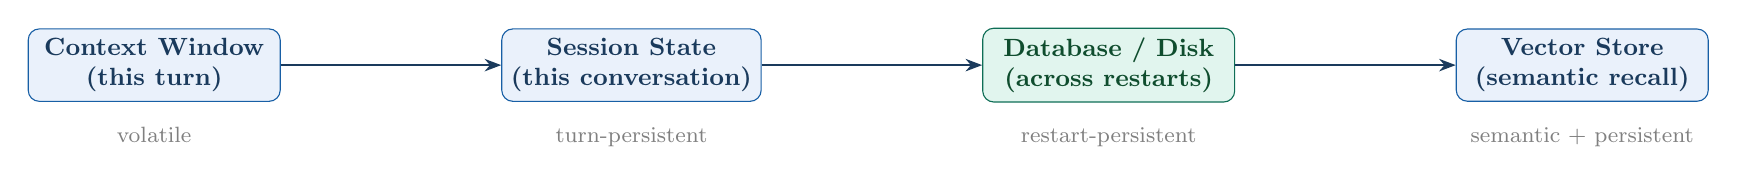
\begin{tikzpicture}[
  node distance=0.8cm and 2.8cm,
  box/.style={rectangle, rounded corners=4pt, draw=theoryborder, fill=theorybg,
               minimum width=3.2cm, minimum height=0.9cm, align=center,
               font=\small\bfseries\color{theoryblue}},
  sbox/.style={rectangle, rounded corners=4pt, draw=practicalborder, fill=practicalbg,
               minimum width=3.2cm, minimum height=0.9cm, align=center,
               font=\small\bfseries\color{practicalgreen}},
  arrow/.style={-{Stealth[length=6pt]}, thick, color=theoryblue},
  label/.style={font=\footnotesize\color{gray}}
]
  \node[box] (ctx)   {Context Window\\(this turn)};
  \node[box, right=of ctx] (sess) {Session State\\(this conversation)};
  \node[sbox, right=of sess] (db)  {Database / Disk\\(across restarts)};
  \node[box, right=of db] (vec)  {Vector Store\\(semantic recall)};

  \draw[arrow] (ctx) -- (sess);
  \draw[arrow] (sess) -- (db);
  \draw[arrow] (db) -- (vec);

  \node[label, below=0.2cm of ctx]  {volatile};
  \node[label, below=0.2cm of sess] {turn-persistent};
  \node[label, below=0.2cm of db]   {restart-persistent};
  \node[label, below=0.2cm of vec]  {semantic + persistent};
\end{tikzpicture}
\end{center}

\begin{description}[leftmargin=3.5cm, style=nextline, font=\bfseries\color{keyterm}]
  \item[Context window] The raw token budget fed to the LLM in a single call. Anything
    outside this window is invisible to the model. This is the agent's \emph{working
    memory} --- extremely fast but strictly size-limited.
  \item[Session state] A key-value scratchpad attached to one conversation thread.
    Survives across turns within a session but, with \texttt{InMemorySessionService},
    is lost on application restart. Analogous to a human's \emph{short-term memory}.
  \item[Persistent storage] A database or file backing a \texttt{DatabaseSessionService}.
    State survives restarts. Analogous to \emph{episodic and semantic long-term memory}.
  \item[Vector store] An embedding database that enables \emph{retrieval-augmented
    generation} (RAG). The agent retrieves semantically relevant past context rather
    than loading the whole history. Day 9 covers this in depth.
\end{description}

% ---------------------------------------------------------------
\subsubsection*{The Four Memory Types}

Classic cognitive science distinguishes four memory types; each maps cleanly onto an ADK pattern:

\medskip
\begin{center}\small
\begin{tabular}{>{\bfseries}p{2.8cm} p{3.8cm} p{4.5cm}}
\toprule
\textbf{Type} & \textbf{What it stores} & \textbf{ADK equivalent} \\
\midrule
Episodic & Specific past events (``what happened'') & \texttt{session.events} --- the ordered list of all turns \\
\addlinespace
Semantic & Facts and knowledge (``what is true'') & Retrieved via RAG / vector store (Day 9) \\
\addlinespace
Procedural & How to perform actions (``how to do it'') & Tool schemas and agent instructions \\
\addlinespace
Working & Currently active information & The context window; \texttt{temp:} state keys \\
\bottomrule
\end{tabular}
\end{center}
\medskip

% ---------------------------------------------------------------
\subsubsection*{The ADK Session Model}

ADK's memory architecture centres on three objects:

\begin{enumerate}[leftmargin=*, itemsep=3pt]
  \item \textbf{Session} (\texttt{google.adk.sessions.Session}) --- the container for
    one conversation thread. Key fields:
    \begin{itemize}[itemsep=1pt]
      \item \texttt{id} --- unique identifier for this thread.
      \item \texttt{app\_name} --- which agent application owns this session.
      \item \texttt{user\_id} --- which user the session belongs to.
      \item \texttt{events} --- chronological list of every interaction (user messages,
        agent responses, tool calls, tool results).
      \item \texttt{state} --- the key-value scratchpad for this conversation.
      \item \texttt{last\_update\_time} --- timestamp of the last event.
    \end{itemize}

  \item \textbf{SessionService} --- the manager responsible for creating, retrieving,
    updating, and deleting sessions. The \texttt{Runner} calls
    \texttt{session\_service.append\_event()} after every turn, which atomically adds
    the event to history \emph{and} applies any \texttt{state\_delta} encoded in that
    event.

  \item \textbf{State} (\texttt{session.state}) --- a flat dictionary. Correctly
    updating state means writing a \texttt{state\_delta} into the event, not mutating
    the dict directly.
\end{enumerate}

\begin{notebox}
\textbf{Official docs:} \url{https://adk.dev/sessions/session/}\\
The session lifecycle diagram at that page shows exactly when
\texttt{create\_session}, \texttt{append\_event}, \texttt{get\_session}, and
\texttt{delete\_session} are called by the Runner.
\end{notebox}

% ---------------------------------------------------------------
\subsubsection*{SessionService Implementations}

\medskip
\begin{center}\small
\begin{tabular}{>{\bfseries}p{3.6cm} p{4cm} p{3.5cm}}
\toprule
\textbf{Service} & \textbf{Persistence} & \textbf{Best for} \\
\midrule
\texttt{InMemorySessionService} & None --- lost on restart & Local dev, unit tests \\
\addlinespace
\texttt{DatabaseSessionService} & Yes --- SQLite/PostgreSQL/MySQL & Self-hosted production \\
\addlinespace
\texttt{VertexAiSessionService} & Yes --- Google Cloud managed & Cloud-native production \\
\bottomrule
\end{tabular}
\end{center}
\medskip

\noindent For today's hands-on you use \texttt{DatabaseSessionService} with SQLite
(\texttt{sqlite+aiosqlite}) so that memory survives restarts --- the key difference
from Day 2's in-memory setup. See:
\url{https://adk.dev/sessions/session/\#databasesessionservice}

% ---------------------------------------------------------------
\subsubsection*{State Keys and Scope Prefixes}

All state is stored as string keys. The prefix of a key determines its scope:

\medskip
\begin{center}\small
\begin{tabular}{>{\ttfamily\bfseries}p{2.5cm} p{3.5cm} p{4.5cm}}
\toprule
\textbf{Prefix} & \textbf{Scope} & \textbf{Example use case} \\
\midrule
(none) & This session only & \texttt{current\_task}, \texttt{booking\_step} \\
\addlinespace
user: & All sessions for this user & \texttt{user:preferred\_currency}, \texttt{user:name} \\
\addlinespace
app: & All users and sessions & \texttt{app:api\_version}, \texttt{app:rate\_limit} \\
\addlinespace
temp: & Current invocation only & \texttt{temp:raw\_api\_response} --- discarded after the turn \\
\bottomrule
\end{tabular}
\end{center}
\medskip

\begin{notebox}
\textbf{Official docs:} \url{https://adk.dev/sessions/state/}\\
The docs confirm that \texttt{temp:} keys are discarded after the invocation
completes and never written to persistent storage, even with
\texttt{DatabaseSessionService}. Use them freely for scratch values within a
single reasoning step.
\end{notebox}

% ---------------------------------------------------------------
\subsubsection*{How to Update State Correctly}

The docs draw a clear distinction between safe and unsafe state mutation:

\begin{description}[leftmargin=4cm, style=nextline, font=\bfseries\color{keyterm}]
  \item[output\_key (easiest)] Set \texttt{output\_key="my\_key"} on the agent. The
    Runner automatically saves the agent's final text response to
    \texttt{session.state["my\_key"]} by encoding a \texttt{state\_delta} in the
    event. Zero extra code required.

  \item[ToolContext.state (in tools)] Inside a tool function, accept a
    \texttt{tool\_context} parameter and write
    \texttt{tool\_context.state["my\_key"] = value}. The ADK framework injects the
    context and captures changes into the next event's \texttt{state\_delta}.

  \item[EventActions.state\_delta (manual)] Construct an \texttt{EventActions} object
    with \texttt{state\_delta=\{...\}} and pass it when calling
    \texttt{session\_service.append\_event()}. Useful for system-level state updates
    that are not driven by the agent's text output.
\end{description}

\begin{warnbox}
\textbf{Never do this:}
\texttt{my\_session.state["key"] = value} directly on a session object obtained
from \texttt{session\_service.get\_session()}.

This bypasses the event system. The change will \emph{not} be saved by
\texttt{DatabaseSessionService} or \texttt{VertexAiSessionService}, it creates
race conditions under concurrency, and it is not auditable. Read \texttt{state}
from a retrieved session; write it only via the three safe methods above.\\[2pt]
Source: \url{https://adk.dev/sessions/state/\#a-warning-about-direct-state-modification}
\end{warnbox}

% ---------------------------------------------------------------
\subsubsection*{Memory Failure Modes}

\medskip
\begin{center}\small
\begin{tabular}{>{\bfseries}p{3.2cm} p{4cm} p{3.8cm}}
\toprule
\textbf{Failure} & \textbf{Cause} & \textbf{Remedy} \\
\midrule
State lost on restart & Using \texttt{InMemory} in production & Switch to \texttt{DatabaseSessionService} \\
\addlinespace
Context overflow & Injecting full history into prompt & Summarise or truncate events before injection \\
\addlinespace
Stale state & Reading from a session object after updates & Always call \texttt{get\_session()} again before reading \\
\addlinespace
Race condition & Directly mutating \texttt{session.state} & Use only \texttt{output\_key} or \texttt{state\_delta} \\
\addlinespace
Missing key error & Using \texttt{\{key\}} in instruction when key absent & Add \texttt{?} suffix: \texttt{\{key?\}} for optional keys \\
\addlinespace
Retrieval noise & Loading all history into context & Use semantic retrieval (RAG) for long conversations \\
\bottomrule
\end{tabular}
\end{center}
\medskip

% ---------------------------------------------------------------
\subsubsection*{Key Concepts Summary}

\begin{enumerate}[leftmargin=*, label=\textbf{\arabic*.}, itemsep=4pt]
  \item \kterm{Session} --- ADK's container for one conversation thread. Holds
    \texttt{id}, \texttt{events}, \texttt{state}, and \texttt{user\_id}.

  \item \kterm{SessionService} --- the manager for session lifecycle.
    \texttt{InMemorySessionService} for dev; \texttt{DatabaseSessionService} for
    persistent local storage; \texttt{VertexAiSessionService} for cloud.

  \item \kterm{session.state} --- a flat key-value scratchpad scoped by prefix:
    no prefix (session), \texttt{user:} (user-wide), \texttt{app:} (app-wide),
    \texttt{temp:} (current invocation only).

  \item \kterm{state\_delta} --- the safe mechanism for writing state. Encoded in
    an \texttt{EventActions} object and applied atomically by \texttt{append\_event}.

  \item \kterm{output\_key} --- the zero-boilerplate shortcut for saving an agent's
    text response directly into state.

  \item \kterm{Memory injection} --- the act of including remembered state or past
    events in the agent's system prompt or context window for a new turn.

  \item \kterm{Retrieval trigger} --- the condition under which the agent decides
    to fetch a past result rather than re-running the tool (Day 9 extends this with
    RAG).
\end{enumerate}

\end{theorybox}

\vspace{1.5em}

% ================================================================
% PRACTICAL SECTION
% ================================================================
\begin{practicalbox}

\subsection*{Task: Add Persistent Session Memory to Your Day 2 Agent}

Today you take the multi-tool agent from Day 2 and give it a proper memory.
The goal is an agent that can recall, across restarts, what it computed in a
previous session --- without re-running the tool.

% ---------------------------------------------------------------
\subsubsection*{Step 1 --- Project setup}

% Official ADK project structure: https://adk.dev/tutorials/multi-tool-agent/#project-structure
% The Day 3 package follows the same conventions as Day 2.

Create a \texttt{day-3/} folder in your repository mirroring Day 2's structure:

\begin{lstlisting}[style=bashstyle]
# From your repo root
mkdir -p day-3/stateful_agent
cd day-3

# Required files
touch stateful_agent/__init__.py
touch stateful_agent/agent.py
touch stateful_agent/tools.py
touch stateful_agent/.env
touch README.md
\end{lstlisting}

Your tree must look like this before writing any code:

\begin{lstlisting}[style=bashstyle]
day-3/                        <-- run `adk web` / `adk run` from HERE
    stateful_agent/
        __init__.py
        agent.py
        tools.py
        .env
    README.md
\end{lstlisting}

\begin{notebox}
\textbf{Same rule as Day 2:} Run \texttt{adk web} and \texttt{adk run} from
\texttt{day-3/} (the parent of the package folder), never from inside
\texttt{stateful\_agent/}. The CLI discovers \texttt{root\_agent} by importing
the package. See \url{https://adk.dev/tutorials/multi-tool-agent/\#run-your-agent}
\end{notebox}

% ---------------------------------------------------------------
\subsubsection*{Step 2 --- Wire up \texttt{\_\_init\_\_.py}}

Exactly as in Day 2 --- one line that makes the package importable:

\begin{lstlisting}[style=bashstyle]
echo "from . import agent" > stateful_agent/__init__.py
\end{lstlisting}

% ---------------------------------------------------------------
\subsubsection*{Step 3 --- Reuse your tools}

Copy \texttt{tools.py} from Day 2 (or create equivalents). The tool functions
themselves need no changes for memory to work --- that is the point. State
persistence is handled entirely at the \texttt{SessionService} layer, not
inside individual tools.

\begin{lstlisting}[style=bashstyle]
cp ../day-2/multi_tool_agent/tools.py stateful_agent/tools.py
\end{lstlisting}

% ---------------------------------------------------------------
\subsubsection*{Step 4 --- Install the async SQLite driver}

% Official ADK requirement: https://adk.dev/sessions/session/#databasesessionservice
% DatabaseSessionService requires an async driver. For SQLite use sqlite+aiosqlite.

\texttt{DatabaseSessionService} requires an \emph{async} database driver.
The official ADK docs specify \texttt{sqlite+aiosqlite} for SQLite:

\begin{lstlisting}[style=bashstyle]
pip install aiosqlite
\end{lstlisting}

\begin{notebox}
\textbf{Why not plain \texttt{sqlite}?} ADK's session service is async
throughout. The synchronous \texttt{sqlite://} driver will raise a
\texttt{MissingGreenlet} error at runtime. Always use
\texttt{sqlite+aiosqlite://} in your connection string.\\[2pt]
Source: \url{https://adk.dev/sessions/session/\#databasesessionservice}
\end{notebox}

% ---------------------------------------------------------------
\subsubsection*{Step 5 --- Write \texttt{agent.py} with \texttt{DatabaseSessionService}}

% Official ADK Session docs: https://adk.dev/sessions/session/
% Official ADK State docs:   https://adk.dev/sessions/state/
%
% Key requirements from the docs:
%   1. agent variable must be named root_agent.
%   2. State is read via session.state (read-only after get_session).
%   3. State is written via output_key or ToolContext.state --- never direct mutation.
%   4. DatabaseSessionService needs sqlite+aiosqlite connection string.

Copy the following into \texttt{stateful\_agent/agent.py}:

\begin{lstlisting}[style=pythonstyle, caption={stateful\_agent/agent.py --- stateful agent with DatabaseSessionService}]
# stateful_agent/agent.py
# Day 3: Memory & State Management
#
# Official ADK Session docs: https://adk.dev/sessions/session/
# Official ADK State docs:   https://adk.dev/sessions/state/

from google.adk.agents import Agent
from google.adk.sessions import DatabaseSessionService

from .tools import calculate, convert_units, format_timestamp

# ----------------------------------------------------------------
# PERSISTENT SESSION SERVICE
# DatabaseSessionService stores state in a local SQLite file.
# The sqlite+aiosqlite:// scheme is required --- plain sqlite:// is
# synchronous and will fail at runtime with ADK.
# Official docs: https://adk.dev/sessions/session/#databasesessionservice
# ----------------------------------------------------------------
DB_URL = "sqlite+aiosqlite:///./day3_memory.db"
session_service = DatabaseSessionService(db_url=DB_URL)

# ----------------------------------------------------------------
# SYSTEM PROMPT
# The {last_result} placeholder is filled from session.state at
# runtime by ADK's instruction templating system.
# If the key is absent (first turn) the ? suffix silences the error.
# Official docs: https://adk.dev/sessions/state/#using-key-templating
# ----------------------------------------------------------------
SYSTEM_PROMPT = """
You are a precise utility assistant with access to three tools:
  - calculate:        for arithmetic and mathematical expressions
  - convert_units:    for physical unit conversions
  - format_timestamp: for converting Unix timestamps to readable dates

Memory available to you:
  Last result stored:  {last_result?}

Rules:
1. Always use a tool when the user's request maps to one.
2. If the user asks to recall a past result, check {last_result?} first.
   Only re-run the tool if the stored result is absent or stale.
3. After every tool call, summarise the result in one sentence starting
   with "Result:". This sentence will be saved as your memory for the
   next session.
"""

# ----------------------------------------------------------------
# ROOT AGENT
# output_key="last_result" tells ADK to save the agent's final
# response text into session.state["last_result"] automatically.
# This is the safest, zero-boilerplate way to write state.
# Official docs: https://adk.dev/sessions/state/#the-easy-way-output_key
# ----------------------------------------------------------------
root_agent = Agent(
    name="stateful_agent",
    model="gemini-2.5-flash",
    description=(
        "A utility agent with persistent memory across restarts."
    ),
    instruction=SYSTEM_PROMPT,
    tools=[calculate, convert_units, format_timestamp],
    output_key="last_result",   # saves final response to state
)
\end{lstlisting}

\begin{notebox}
\textbf{What \texttt{output\_key} does under the hood:} After every turn, the
\texttt{Runner} encodes the agent's final text as a \texttt{state\_delta} inside
the event's \texttt{EventActions} and calls
\texttt{session\_service.append\_event()}. The \texttt{DatabaseSessionService}
then writes the delta to SQLite. On the next turn, \texttt{get\_session()}
returns the updated state, which ADK injects into \texttt{\{last\_result\}} in
your instruction. No extra code needed on your part.
\end{notebox}

% ---------------------------------------------------------------
\subsubsection*{Step 6 --- Configure \texttt{.env}}

Same as Day 2. Open \texttt{stateful\_agent/.env}:

\begin{lstlisting}[style=bashstyle, caption={stateful\_agent/.env}]
GOOGLE_GENAI_USE_VERTEXAI=FALSE
GOOGLE_API_KEY=PASTE_YOUR_ACTUAL_API_KEY_HERE
\end{lstlisting}

Get a free key at \url{https://aistudio.google.com/apikey}.

% ---------------------------------------------------------------
\subsubsection*{Step 7 --- Run with \texttt{adk web} and test memory persistence}

% Official run instructions: https://adk.dev/tutorials/multi-tool-agent/#run-your-agent

From \texttt{day-3/} (the parent of the package folder):

\begin{lstlisting}[style=bashstyle]
adk web
\end{lstlisting}

Open \texttt{http://localhost:8000}, select \textbf{stateful\_agent} from the
dropdown, and run this sequence:

\begin{enumerate}[leftmargin=*, itemsep=2pt]
  \item Ask: \texttt{What is sqrt(144) + 20\% of 500?}
  \item Confirm the agent calls \texttt{calculate} and gives you the result.
  \item \textbf{Stop \texttt{adk web}} (Ctrl+C) --- this simulates a restart.
  \item Run \texttt{adk web} again and open a \emph{new} chat in the same session.
  \item Ask: \texttt{What was the last result you computed?}
  \item The agent should answer from memory without calling any tool.
\end{enumerate}

\begin{notebox}
\textbf{Session ID matters:} The agent will only recall memory if you use the
same \texttt{session\_id}. In \texttt{adk web}, each browser tab maintains its
session. To replay the same session after a restart, note the session ID shown
in the Events tab and reuse it. Alternatively use \texttt{adk run} with a
fixed session ID (see Step 8).
\end{notebox}

% ---------------------------------------------------------------
\subsubsection*{Step 8 --- Test persistence with a script}

For reproducible demos, write a small script that explicitly creates and reuses
a named session. Save as \texttt{day-3/demo\_memory.py}:

\begin{lstlisting}[style=pythonstyle, caption={day-3/demo\_memory.py --- demonstrate cross-restart recall}]
# demo_memory.py  (run from day-3/ with: python demo_memory.py)
# Demonstrates that DatabaseSessionService preserves state across
# simulated restarts by reusing a fixed session_id.
#
# Official Session docs: https://adk.dev/sessions/session/

import asyncio
from google.adk.runners import InMemoryRunner
from google.genai import types

# Import the package the same way the CLI does
from stateful_agent.agent import root_agent, session_service

APP_NAME   = "stateful_demo"
USER_ID    = "demo_user"
SESSION_ID = "persistent_session_001"  # fixed ID so we can reuse it


async def send(runner, session_id: str, query: str) -> str:
    """Send a query and return the agent's final text response."""
    content = types.Content(
        role="user",
        parts=[types.Part(text=query)],
    )
    response = ""
    async for event in runner.run_async(
        user_id=USER_ID,
        session_id=session_id,
        new_message=content,
    ):
        if event.is_final_response() and event.content:
            response = event.content.parts[0].text
    return response


async def main() -> None:
    # Use the DatabaseSessionService from agent.py so state is shared
    runner = InMemoryRunner(
        agent=root_agent,
        app_name=APP_NAME,
        session_service=session_service,   # <-- persistent service
    )

    # Create or re-use the session
    try:
        session = await session_service.get_session(
            app_name=APP_NAME,
            user_id=USER_ID,
            session_id=SESSION_ID,
        )
        if session is None:
            raise ValueError("Session not found")
        print(f"[Resuming existing session: {SESSION_ID}]")
    except Exception:
        session = await session_service.create_session(
            app_name=APP_NAME,
            user_id=USER_ID,
            session_id=SESSION_ID,
        )
        print(f"[Created new session: {SESSION_ID}]")

    print(f"State at start: {session.state}\n")

    # --- Turn 1: compute something ---
    q1 = "Convert 100 km to miles."
    print(f"User:  {q1}")
    r1 = await send(runner, session.id, q1)
    print(f"Agent: {r1}\n")

    # --- Turn 2: recall without re-running the tool ---
    q2 = "What was the last result you computed? Do not call any tool."
    print(f"User:  {q2}")
    r2 = await send(runner, session.id, q2)
    print(f"Agent: {r2}\n")

    # --- Inspect persisted state ---
    updated = await session_service.get_session(
        app_name=APP_NAME,
        user_id=USER_ID,
        session_id=SESSION_ID,
    )
    print(f"Persisted state: {updated.state}")
    print("\nRun this script again and the agent will recall the result "
          "from SQLite without re-running the tool.")


if __name__ == "__main__":
    asyncio.run(main())
\end{lstlisting}

Run it twice in a row:

\begin{lstlisting}[style=bashstyle]
python demo_memory.py   # First run: creates session, computes result
python demo_memory.py   # Second run: resumes session, recalls from state
\end{lstlisting}

On the second run the agent should answer the recall question from
\texttt{last\_result} in state without invoking \texttt{convert\_units} again.
Document what you observe in \texttt{README.md}.

% ---------------------------------------------------------------
\subsubsection*{Step 9 --- Write state from inside a tool (advanced)}

% Official ToolContext docs: https://adk.dev/sessions/state/#via-callbackcontext-or-toolcontext
%
% Tools can write to state by accepting tool_context as a parameter.
% ADK injects the context automatically when the parameter is named
% tool_context and typed as ToolContext.

The \texttt{output\_key} approach saves the agent's \emph{final text}. Sometimes
you want to save a structured value (e.g., a raw dict) from \emph{inside} the
tool. ADK provides \texttt{ToolContext} for this:

\begin{lstlisting}[style=pythonstyle, caption={Saving structured data from inside a tool via ToolContext}]
# Add to stateful_agent/tools.py
# Official ToolContext docs:
# https://adk.dev/sessions/state/#via-callbackcontext-or-toolcontext

from google.adk.tools import ToolContext

def convert_units_stateful(
    value: float,
    from_unit: str,
    to_unit: str,
    tool_context: ToolContext,       # ADK injects this automatically
) -> dict:
    """
    Converts a value between physical units and stores the raw result
    in session state for later recall. Use this when the user asks to
    convert between km and miles, kg and lbs, Celsius and Fahrenheit,
    or similar unit conversions. Do NOT use for currency conversion.

    Args:
        value:        The numeric value to convert.
        from_unit:    The source unit (e.g. 'km', 'kg', 'celsius').
        to_unit:      The target unit (e.g. 'miles', 'lbs', 'fahrenheit').
        tool_context: Injected by ADK -- do not pass manually.

    Returns:
        A dict with 'result' (float) and 'unit' (str), or 'error' (str).
    """
    conversions = {
        ("km", "miles"):           lambda x: x * 0.621371,
        ("miles", "km"):           lambda x: x * 1.60934,
        ("kg", "lbs"):             lambda x: x * 2.20462,
        ("lbs", "kg"):             lambda x: x * 0.453592,
        ("celsius", "fahrenheit"): lambda x: (x * 9 / 5) + 32,
        ("fahrenheit", "celsius"): lambda x: (x - 32) * 5 / 9,
        ("meters", "feet"):        lambda x: x * 3.28084,
        ("feet", "meters"):        lambda x: x * 0.3048,
    }
    key = (from_unit.lower(), to_unit.lower())
    if key in conversions:
        result = {
            "result":   round(conversions[key](value), 4),
            "unit":     to_unit,
            "original": f"{value} {from_unit}",
        }
        # Write to state via ToolContext -- safe, tracked by append_event
        # The key has no prefix, so it is session-scoped.
        tool_context.state["last_conversion"] = result
        return result
    return {"error": f"Conversion from {from_unit} to {to_unit} not supported."}
\end{lstlisting}

\begin{notebox}
ADK recognises the \texttt{tool\_context} parameter by name and type and injects
the current \texttt{ToolContext} automatically. You never pass it manually.
Writing \texttt{tool\_context.state["key"] = value} is the correct way to store
structured data from inside a tool. The framework adds this to the event's
\texttt{state\_delta}, so it is properly persisted by \texttt{DatabaseSessionService}.
\end{notebox}

% ---------------------------------------------------------------
\subsubsection*{Step 10 --- Document your observations and commit}

After running both \texttt{adk web} and \texttt{demo\_memory.py}, write a
short \texttt{README.md} covering:

\begin{itemize}[leftmargin=*, itemsep=2pt]
  \item Which session service you used and why.
  \item What \texttt{session.state} contained after the first run (paste the
    printed output).
  \item Whether the agent recalled the result correctly on the second run.
  \item One failure mode you encountered or deliberately triggered (e.g.,
    what happens if you delete the \texttt{.db} file between runs?).
\end{itemize}

Then commit:

\begin{lstlisting}[style=bashstyle]
cd ..   # back to repo root
git add day-3/
git commit -m "Day 3: stateful agent with DatabaseSessionService + memory demo"
git push
\end{lstlisting}

\medskip

\begin{stretchbox}
\textbf{Stretch Goal:} Implement a simple semantic retrieval layer using
\texttt{numpy} cosine similarity. Store each tool result as an embedding
(use \texttt{sentence-transformers} or a small Gemini embedding call) in a
list under \texttt{session.state["embedding\_store"]}. On each turn, embed
the user query and retrieve the most similar past result. This is a
hand-rolled preview of the RAG pipeline you will build on Day 9.
\end{stretchbox}

\end{practicalbox}

\vspace{1.5em}

% ================================================================
% DELIVERABLE
% ================================================================
\begin{delivbox}
\begin{itemize}[leftmargin=*, itemsep=3pt]
  \item Stateful agent committed to \texttt{day-3/} on GitHub, using
    \texttt{DatabaseSessionService} with a local SQLite file.
  \item \texttt{demo\_memory.py} demonstrating cross-restart recall --- run it
    twice and paste the second-run output in \texttt{README.md}.
  \item \texttt{README.md} documenting: which service was used, the persisted
    state contents, and one failure mode observed.
  \item (Stretch) Semantic similarity retrieval implemented and tested with at
    least three stored past results.
\end{itemize}
\end{delivbox}

\vspace{1.5em}

% ================================================================
% SELF-CHECK QUESTIONS
% ================================================================
\section{Self-Check Questions}

\begin{enumerate}[leftmargin=*, label=\textbf{Q\arabic*.}, itemsep=6pt]
  \item What is the difference between \texttt{InMemorySessionService} and
    \texttt{DatabaseSessionService}? When would you choose each?

  \item Explain what happens to a \texttt{temp:} prefixed key after a turn
    completes. Give a concrete example of when you would use it.

  \item You write \texttt{retrieved\_session.state["count"] += 1} directly in
    your application code. What are two specific ways this can break your agent
    in production?

  \item Your agent instruction includes \texttt{\{user\_name\}}. On the first
    turn, no one has set that key yet. What error occurs, and how do you fix it
    without removing the placeholder?

  \item Walk through what \texttt{output\_key="last\_result"} causes ADK to do,
    step by step, from when the agent produces its response to when the value is
    readable in the next turn's context.

  \item A user asks your agent: ``What did you calculate last time?'' --- but
    this is a new session (different \texttt{session\_id}). The agent has no
    memory of the previous result. What architectural options do you have to
    solve this?
\end{enumerate}

\vspace{1.5em}

% ================================================================
% CONNECTIONS TO THE BROADER ROADMAP
% ================================================================
\section{Connections to the Broader Roadmap}

\begin{table}[h!]
\centering
\small
\begin{tabular}{>{\bfseries}p{2.5cm} p{4.5cm} p{5cm}}
\toprule
\textbf{Today} & \textbf{This leads to\ldots} & \textbf{Why it matters} \\
\midrule
DatabaseSessionService & Day 4--6: FinSight Agent & FinSight needs persistent state to track portfolio queries across sub-agents. \\
\addlinespace
output\_key pattern & Day 5--6: Structured reports & Every sub-agent in FinSight writes its output to a named state key for the orchestrator to read. \\
\addlinespace
State prefixes & Day 8: ClinAssist safety layer & User-scoped state (\texttt{user:}) persists patient preferences safely across sessions. \\
\addlinespace
Retrieval triggers & Day 9: RAG pipelines & Today's ``check state before re-running'' logic is the manual precursor to semantic retrieval. \\
\addlinespace
Memory failure modes & Day 6: Evaluation harness & Stale state and context overflow are failure categories your eval harness must detect. \\
\bottomrule
\end{tabular}
\caption{How Day 3 concepts thread through the sprint}
\end{table}

% ================================================================
% QUICK REFERENCE
% ================================================================
\section{Quick Reference}

\subsection*{Glossary}

\begin{description}[leftmargin=4.5cm, style=nextline, font=\bfseries\color{keyterm}]
  \item[Session] ADK's container for one conversation thread: \texttt{id},
    \texttt{user\_id}, \texttt{app\_name}, \texttt{events}, \texttt{state}.
  \item[SessionService] The manager for session lifecycle. Three implementations:
    \texttt{InMemory}, \texttt{Database}, \texttt{VertexAI}.
  \item[session.state] A flat serialisable key-value dict scoped by key prefix.
    Read safely from a retrieved session; write only via safe methods.
  \item[state\_delta] The dict of changes encoded in an \texttt{EventActions}
    object and applied atomically by \texttt{append\_event}.
  \item[output\_key] An \texttt{Agent} parameter that instructs the Runner to
    write the agent's final text response to a named state key automatically.
  \item[ToolContext] An ADK object injected into a tool function when the
    parameter is named \texttt{tool\_context}. Exposes \texttt{.state} for
    safe state writes from inside tools.
  \item[Memory injection] Including stored state or summarised history in an
    agent's instruction or context window for the current turn.
  \item[Retrieval trigger] A condition that causes the agent to look up past
    results rather than re-executing a tool.
  \item[Episodic memory] The agent's record of specific past events, stored in
    \texttt{session.events}.
  \item[Semantic memory] Factual knowledge retrieved on demand via a vector
    store (RAG). Covered on Day 9.
\end{description}

\subsection*{State-Writing Pattern Cheat Sheet}

\begin{table}[h!]
\centering
\small
\begin{tabular}{>{\bfseries}p{3.5cm} p{4cm} p{4cm}}
\toprule
\textbf{Method} & \textbf{When to use} & \textbf{Code} \\
\midrule
\texttt{output\_key} & Save agent's final text response & \texttt{Agent(..., output\_key="key")} \\
\addlinespace
\texttt{ToolContext.state} & Save structured data from a tool & \texttt{tool\_context.state["key"] = val} \\
\addlinespace
\texttt{EventActions.state\_delta} & System-level or batch updates & \texttt{EventActions(state\_delta=\{...\})} \\
\addlinespace
Direct mutation & \textbf{Never} --- unsafe & \texttt{session.state["k"] = v}  \textbf{(DON'T)} \\
\bottomrule
\end{tabular}
\caption{When to use each state-writing method}
\end{table}

\subsection*{Key ADK Patterns Today}

\begin{lstlisting}[style=pythonstyle]
# Official docs: https://adk.dev/sessions/session/
#                https://adk.dev/sessions/state/

# 1. Persistent session service (sqlite+aiosqlite required)
from google.adk.sessions import DatabaseSessionService
session_service = DatabaseSessionService(
    db_url="sqlite+aiosqlite:///./my_agent.db"
)

# 2. Agent with output_key saves final text to state automatically
from google.adk.agents import Agent
root_agent = Agent(
    name="stateful_agent",
    model="gemini-2.5-flash",
    description="...",
    instruction="Previous result: {last_result?}",  # {key?} = optional
    tools=[...],
    output_key="last_result",
)

# 3. Tool writing structured data to state via ToolContext
from google.adk.tools import ToolContext

def my_tool(param: str, tool_context: ToolContext) -> dict:
    result = {"value": 42, "param": param}
    tool_context.state["my_tool_result"] = result  # safe write
    return result

# 4. Read state from a retrieved session (read-only)
session = await session_service.get_session(
    app_name=APP_NAME, user_id=USER_ID, session_id=SESSION_ID
)
print(session.state)   # read
# session.state["key"] = val  <-- NEVER do this
\end{lstlisting}

\vfill
\noindent\rule{\textwidth}{0.4pt}\\
{\small\textcolor{gray}{AI Workflow Integration Specialist --- Week 1 Study Notes \hfill Day 3 of 14}}

\end{document}
